\normalfalse \difficiletrue \tdifficilefalse
\correctionfalse

%\UPSTIidClasse{11} % 11 sup, 12 spé
%\newcommand{\UPSTIidClasse}{12}

\exer{Mouvement RT -- RSG  $\star\star$ \label{CIN:01:B2:13:PTSI:09}}
\setcounter{question}{0}\marginnote{\xpComp{CIN}{01}}%\UPSTIcompetence[2]{B2-13}
\index{Compétence B2-13-PTSI}
\index{Mécanisme à 1 rotations, 1 translation et RSG}
\ifcorrection
\else
\marginnote{\textbf{Pas de corrigé pour cet exercice.}}
\fi

\ifprof
\else
Soit le mécanisme suivant. 
\begin{marginfigure}
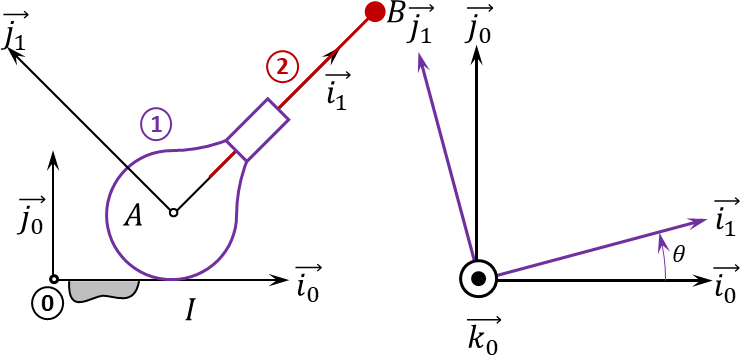
\includegraphics[width=\linewidth]{09_RT_RSG_01}
\end{marginfigure}
\fi


\question{Réaliser le paramétrage du mécanisme.}
\ifprof ~\\

\else
\fi

\question{Donner le torseur cinématique $\torseurcin{V}{2}{0}$ au point $B$.}
\ifprof ~\\
\else
\fi

\question{Déterminer $\vectg{B}{2}{0}$.}
\ifprof ~\\

\else
\fi

\ifprof
\else
\footnotesize

\normalsize
\marginnote{Corrigé voir \ref{CIN:01:B2:13:PTSI:09}.}

\fi